% This section describes the design of the memory system model. How host target
% decoupling is achieved. What configurations are available.
\PNAME is a \textit{generator}, written in Chisel~\cite{Chisel}, that can
elaborate \textit{instances} from a space of possible parameterizations.
Instances themselves model a space of different memory systems: the user picks the
final target-design point by programming the instance's configuration registers
at runtime.

As input, \PNAME accepts a parameterization that constrains features
of the instance, such as its interface widths, the maximum number of
outstanding requests it must support, and the type of memory system the
instance will model (a \emph{timing-model class}). As output, \PNAME generates
an instance RTL module and memory map of its host configuration registers. These
registers control timing parameters; their values can be modified at runtime
to reconfigure the instance without needing to recompile the FPGA bitstream.

\section{Instance Organization}

\begin{figure}[t]
	\centering
	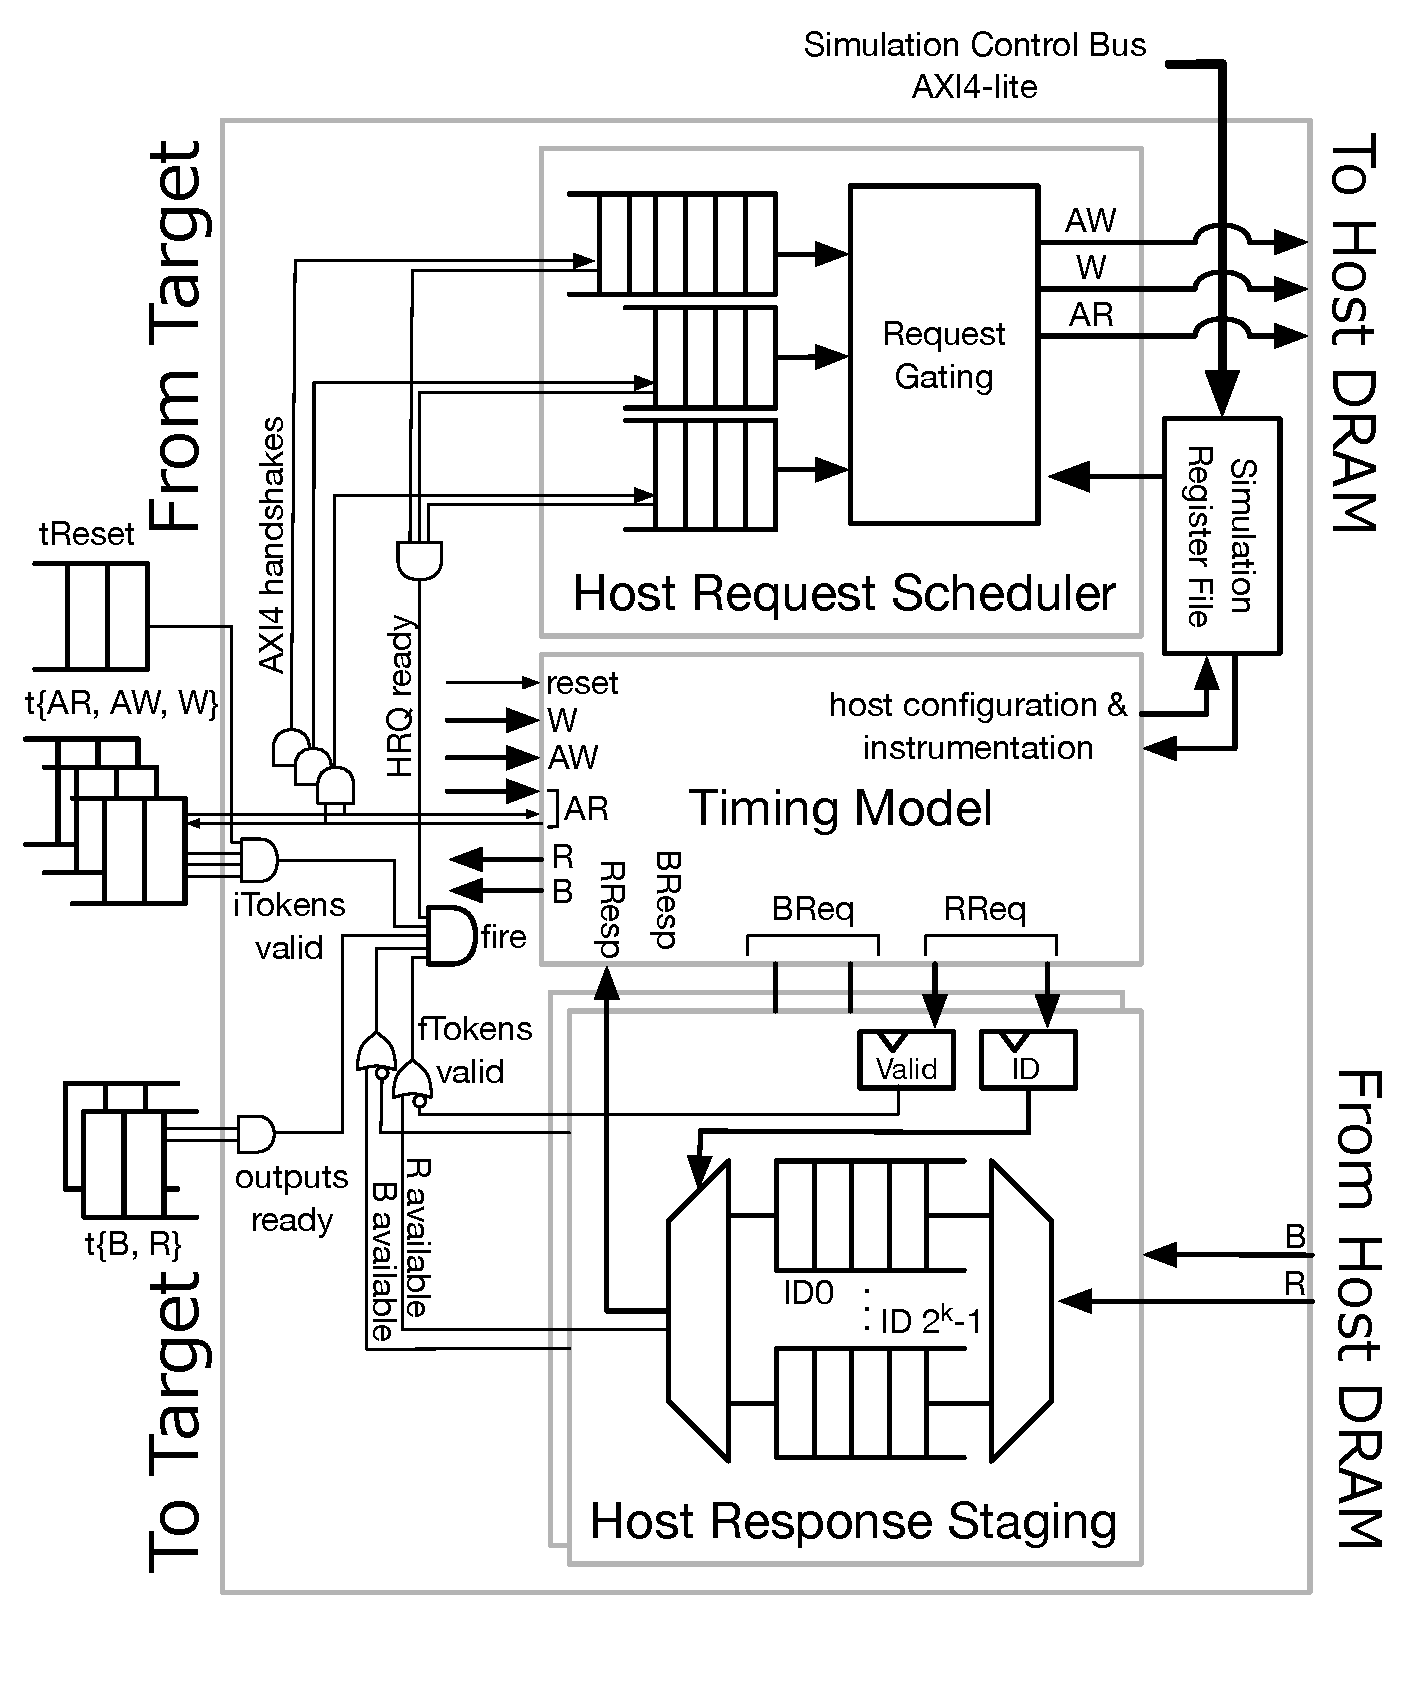
\includegraphics[width=0.8\textwidth]{figures/memory-model-block-diagram.pdf}
     % graffle2pdf -c full midas-graphics/graffle/memory-model-block-diagram.graffle figures/memory-model-block-diagram.pdf
    \caption{A block diagram of a \PNAME instance, with all signals
    that may stall timing model execution illustrated.}
	\label{fig:timing-model}
\end{figure}

The block diagram of an instance is shown in Figure~\ref{fig:timing-model}.
Instances operate by using the FPGA host's DRAM as a backing store.  Target
requests carried in simulation tokens are snooped by the \emph{host-request
scheduler}, which issues them to the host memory system.  Responses from the
host memory system are subsequently buffered in the \emph{host-response
staging} modules. In parallel, the \emph{timing model}, a simulation model
transformed from target-time RTL using a FAME-1 transform, consumes input
tokens and generates output tokens. When the timing model wishes to release a
valid memory-response token, it queries the host-response staging module for
the corresponding host response. If the host memory system has not yet responded,
\texttt{targetFire} is de-asserted, preventing token flow and
ultimately stalling the simulator. We describe this mechanism in greater detail in
the next section~(\ref{sec:memory-model-operation}).

The host-request scheduler and host-response staging modules, together with the
FPGA-host DRAM, constitute the functional model of an instance.  Timing models
are written in target-time RTL and have three interfaces:

\begin{enumerate}
    \item An AXI4 port through which the model receives memory requests from the rest of the target.
    \item Two functional-model request ports~(BREQ \& RREQ) through which the
        timing model fetches data for target responses from the host-response
        staging module. Responses are carried by the next tokens~(fTokens)
        generated by the host-response staging unit.
    \item A host-configuration port that carries the timing parameters of the
        model and records instrumentation data.
\end{enumerate}

During instance generation, \PNAME binds the host-configuration port to memory-mapped
registers on the simulation bus. It then FAME-1-transforms the timing model, connects it to
token queues, and binds the \texttt{targetFire} signal, which is asserted when all of the following
conditions hold:

\begin{enumerate}
    \item All input tokens are present~(\textit{iTokens valid} in Figure~\ref{fig:timing-model}).
    \item All output queues are ready~(\textit{outputs ready}).
    \item The host-request scheduler can accept a request~(\textit{HRQ ready}).
    \item All host-response tokens are present~(\textit{fTokens valid}).
\end{enumerate}

\section{Operation}\label{sec:memory-model-operation}

\begin{figure*}[t]
	\centering
    \begin{subfigure}[t]{0.23\textwidth}
        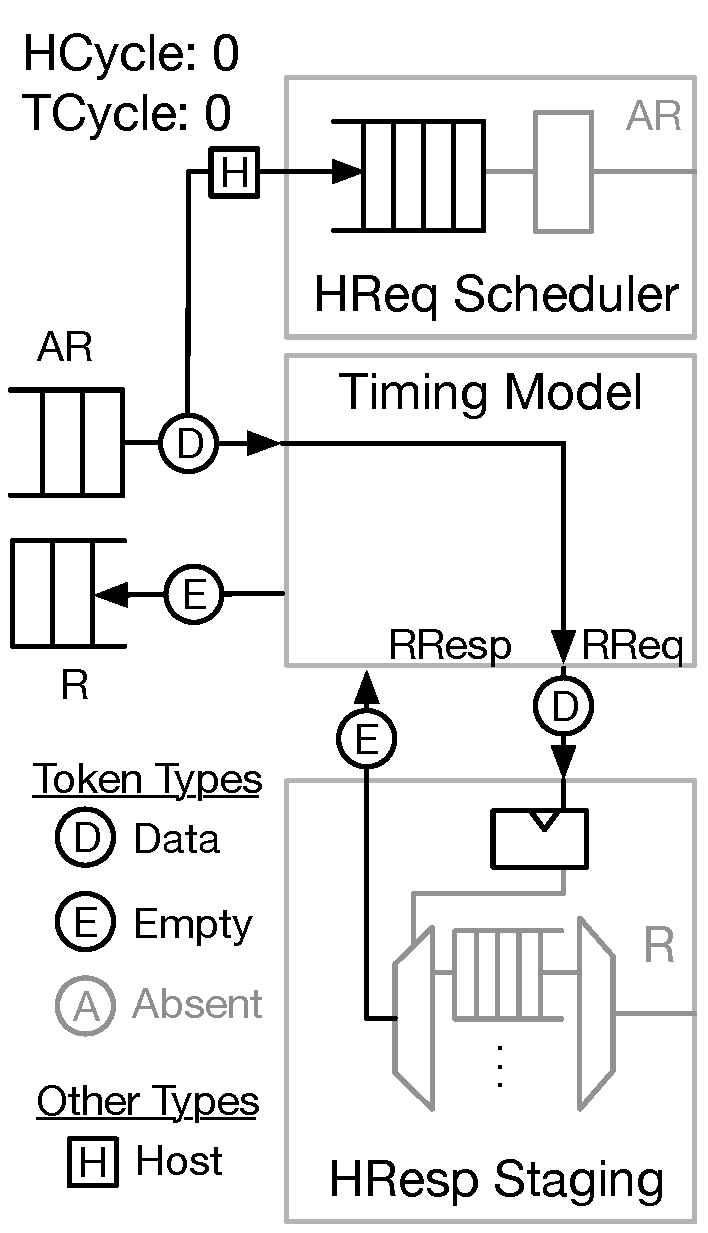
\includegraphics[width=\columnwidth]{figures/model-operation-1.pdf}
        % graffle2pdf -c 1 midas-graphics/graffle/memory-model-operation.graffle figures/model-operation-1.pdf
        \caption{}
        \label{fig:model-operation-1}
    \end{subfigure}
    \begin{subfigure}[t]{0.24\textwidth}
        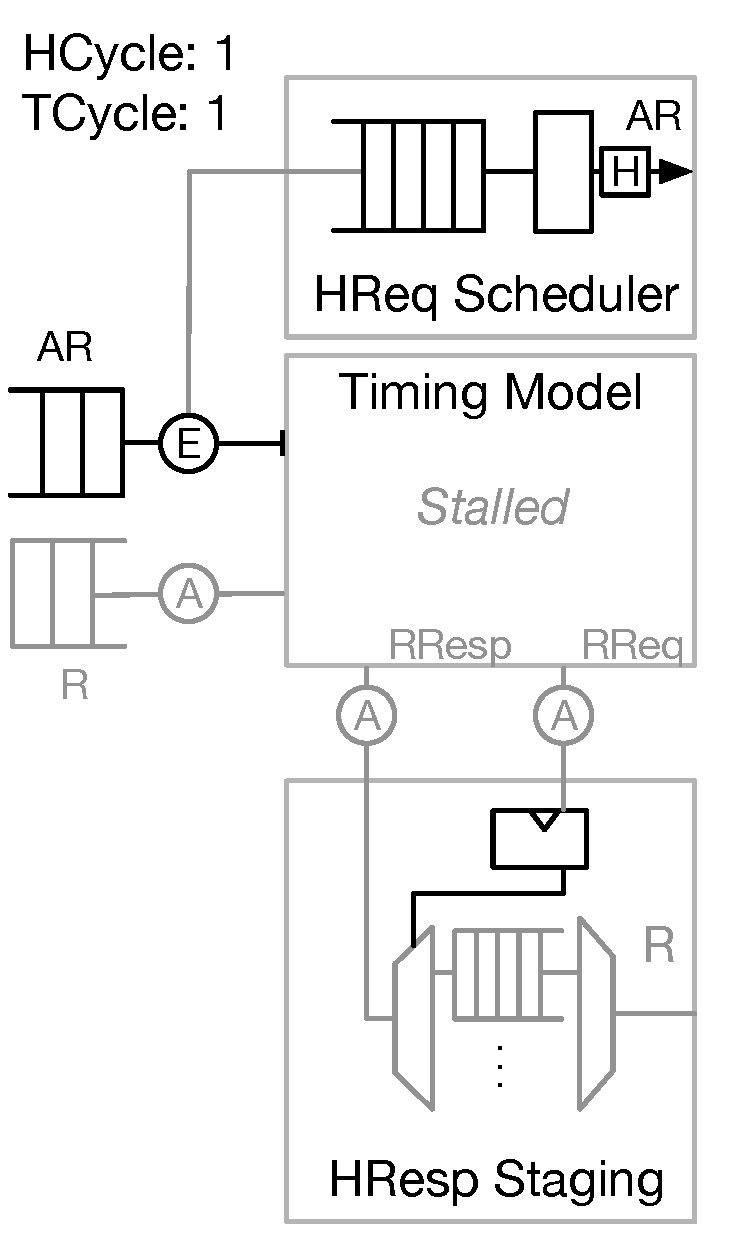
\includegraphics[width=\columnwidth]{figures/model-operation-2.pdf}
        % graffle2pdf -c 2 midas-graphics/graffle/memory-model-operation.graffle figures/model-operation-2.pdf
        \caption{}
        \label{fig:model-operation-2}
    \end{subfigure}
    \begin{subfigure}[t]{0.24\textwidth}
        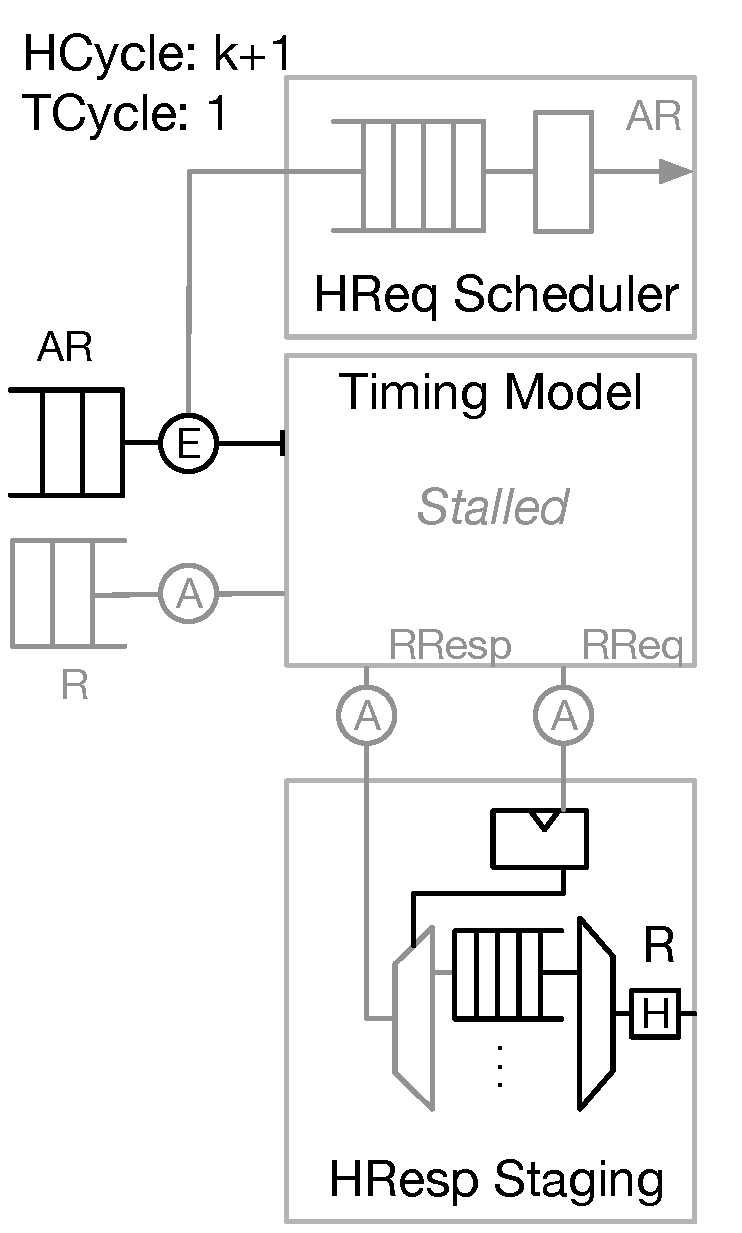
\includegraphics[width=\columnwidth]{figures/model-operation-3.pdf}
        % graffle2pdf -c 3 midas-graphics/graffle/memory-model-operation.graffle figures/model-operation-3.pdf
        \caption{}
        \label{fig:model-operation-3}
    \end{subfigure}
    \begin{subfigure}[t]{0.23\textwidth}
        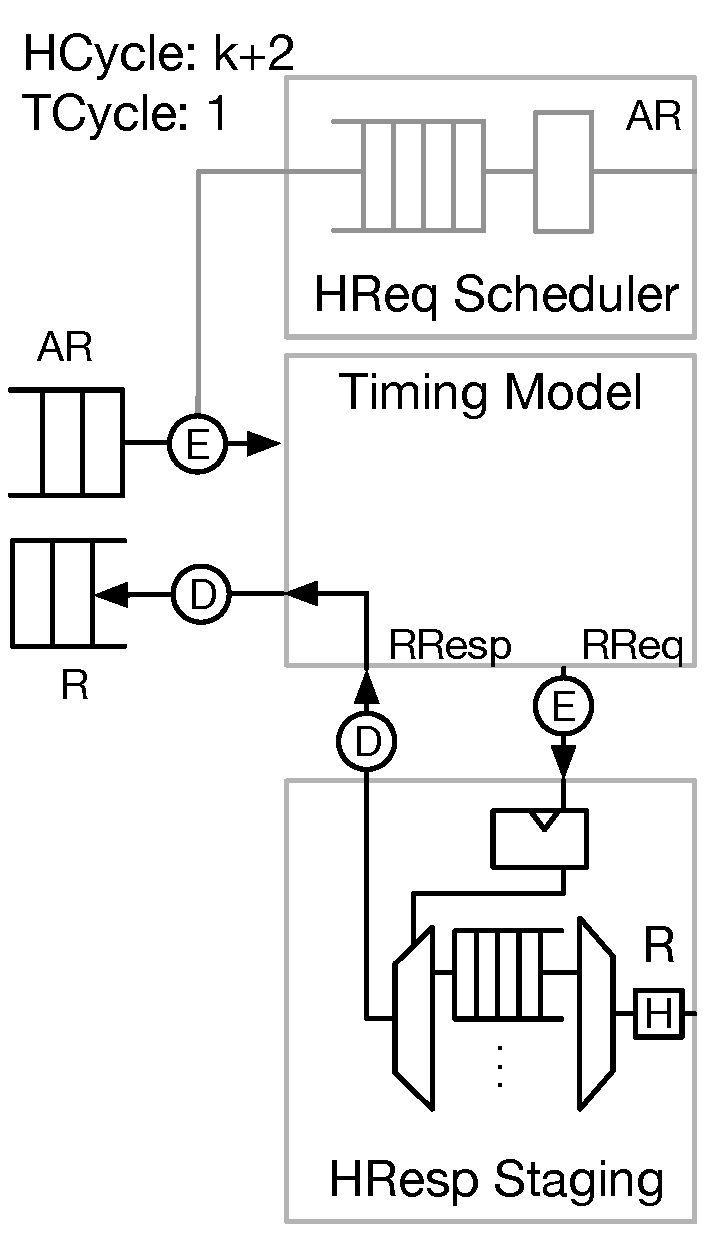
\includegraphics[width=\columnwidth]{figures/model-operation-4.pdf}
        % graffle2pdf -c 4 midas-graphics/graffle/memory-model-operation.graffle figures/model-operation-4.pdf
        \caption{}
        \label{fig:model-operation-4}
    \end{subfigure}
	\centering
    \caption{A \PNAME instance simulating a single-target-cycle read. Data
    tokens carry target transactions~(their target-valid bit is set) whereas
    empty tokens do not carry a target transaction.}
    \label{fig:model-operation}
\end{figure*}

To demonstrate how \PNAME instances operate, let us consider an instance with a
single-cycle-memory timing-model. This is depicted in Figures~\ref{fig:model-operation-1}-\ref{fig:model-operation-4}.

Suppose we have reached the first read request issued to the memory
system~(Figure~\ref{fig:model-operation-1}).  Let this be host and target cycle
0. When the timing model accepts this request, it is snooped by
host-request scheduler.  Simultaneously, the timing model makes a request
to host-response staging module as it needs to reply to the read in the next
target cycle.

In host cycle 2~(Figure~\ref{fig:model-operation-2}), the host-response staging module cannot produce
the associated host response, since it has yet to be issued, and so generates
no fToken, stalling the timing model. In parallel, the host-request scheduler
issues the required read to the host memory system.
While the host-response staging module waits, the timing model
stalls. If the host memory system responds in $K$ cycles, at host
cycle $K+1$~(Figure~\ref{fig:model-operation-3}), that response is received.

In cycle $K+2$~(Figure~\ref{fig:model-operation-4}), the host-response staging module produces an
output token, targetFire is asserted, and target cycle 1 executes. Here the
timing model forwards the data directly into its output token.
From the target's perspective, the read occurred in a single cycle, however,
the cycle was executed with an FMR of $K+2$.  As the latency of the
target increases, FMR decreases and approaches unity.  If the
target memory system is strictly slower the host memory system, the instance
executes at unity FMR.

\section{Functional Model Configuration}\label{egress}
Our design allows both the host memory system and the timing model to reorder
responses; the host-staging unit implements a set of virtual queues for each
AXI4 channel. Each queue represents the FIFO ordering within a single channel
ID. The size of the functional model is sensitive to the maximum number of reads
and writes it must accept, the maximum number of transactions that can be in
flight on the same ID, and the maximum request lengths. For small degrees of ID
reuse, or small numbers of outstanding requests, the memory system model
implements each virtual queue as a physical queue, and aggregates them together in one dual-ported
BRAM~\cite{LIFPGADesign}. For greater numbers of AXI IDs or greater degrees of ID
reuse, it dynamically assigns entries within block RAMs, and maintains a
hardware linked list to track to read-response order in a given ID.

\section{Providing Deterministic Functional-Model Behavior}
By default, instances forward target requests directly to the host-memory
system, under the assumption there will never be reads and writes to the same
address in flight\footnote{In AXI4, the value a read returns when a write to
the same address is in-flight is implementation defined.}. When a buggy target
exhibits this behavior, the host memory-system is free to reorder these
requests, introducing non-determinism. To help debug targets that behave this
way, the host-request scheduler provides a strict mode in which it orders reads
and writes---issuing writes only when no reads are in flight, and reads only
when there are no writes in flight.

\section{General-Purpose Timing-Model Classes}\label{sec:timing_model}

\PNAME provides two simple, general-purpose timing-model-classes that can be used to
model large off-chip memory systems. The first is a \emph{latency-bandwidth
pipe}~(LBP) that applies independently programmable latencies to read and write
requests and will not accept any new requests beyond a programmable limit. The
second is a \emph{bank-conflict} model, which adds a penalty of $max(0, t_{CP} -
t_{\Delta})$ cycles to a base latency if the bank was used
$t_{\Delta}$ cycles prior, where $t_{CP}$ is the maximum conflict penalty.
These models were validated in trace-driven RTL simulation against
software golden models which match their cycle-by-cycle behavior exactly.  We
give the FPGA resource utilization for a handful of
instances in Table~\ref{tbl:lbp-model-resources}\footnote{We
used Vivado 2017.1, targeting the XCVU9P-FLGB2104-2-i device present on F1
instances. We registered all I/O, and overconstrained the design
to \wunits{400}{MHz} to obtain a best-case $f_{MAX}$. We exclude memory
LUTs~(lightly used) and DSP48s~(unused).}.

\begin{table}[htb]
\centering
    \begin{tabular}{c c c c c }
	\hline
        \textbf{Example Instance} & Logic LUTs & FFs & BRAM & $f_{MAX}$ \\
	\hline
        8 read, 8 write & 1337 & 972 & 3 &  281 \\
        32 read, 32 write & 2119 & 1500 & 1 & 264 \\
        Above w/ no ID reuse & 1289 & 873 & 1 & 317 \\
	\hline
	\end{tabular}
    \caption{Resource counts and best-case $f_{MAX}$~(MHz) for three different
    LBP models (maximum AXI4 burst length of 8 beats). Supporting more concurrent transactions~(row 2) requires a larger
    functional model; this can be mitigated by giving the generator hints~(row 3).}
\label{tbl:lbp-model-resources}
\end{table}

\section{Composable Last-Level-Cache Model}
All timing model classes can be generated with a single-banked, write-back,
last level cache~(LLC) model with a random replacement policy.  Since we can
reuse the same functional model, the model only instantiates tag and metadata
arrays, letting us model an LLC that would be too
large to fit on the FPGA. \PNAME LLC models have a runtime-configurable number of sets
and MSHRs, associativity, and line size. Refills from the backing memory model
are prioritized over reads over writes. Reads or writes made to a set with a
pending writeback or refill are interlocked.  We make the cache composable with
all other timing-models by implementing an additional internal AXI4
bus~(stripped of its data fields). We give the FPGA resource utilization for a
handful of LBP-backed LLC instances in
Table~\ref{tbl:llc-model-resources}.
\begin{table}[htb]
\centering
    \begin{tabular}{c c c c c}
	\hline
        \textbf{Example Instance} & Logic LUTs & FFs & BRAM & $f_{MAX}$ \\
	\hline
        4 MiB, 16 ways & 2166 & 1240 & 27 & 222 \\
        4 MiB, 8 ways  & 2265 & 1272 & 39 & 220 \\
        4 MiB, direct mapped & 1848 & 1241 & 34 & 242 \\
        64 MiB, 8 ways & 2545 & 1426 & 251 & 152 \\
	\hline
	\end{tabular}
    \caption{Resource counts and best-case $f_{MAX}$~(MHz) for four different
    LBP-backed LLC models, labeled with the largest capacity and associativity they can model~(128B cache lines).}
\label{tbl:llc-model-resources}
\end{table}

We validated the LLC model in RTL simulation backed with a latency bandwidth
pipe. We generated trace-based microbenchmarks and measured cache behavior
for a set of generated instances programmed with runtime settings.
